%%%%%%%%%%%%%%%%%%%%%%%%%%%%%%%%%%%%
% Slide options
%%%%%%%%%%%%%%%%%%%%%%%%%%%%%%%%%%%%

% Option 1: Slides with solutions

\documentclass[slidestop,compress,mathserif]{beamer}
\newcommand{\soln}[1]{\textit{#1}}
\newcommand{\solnGr}[1]{#1}

% Option 2: Handouts without solutions

%\documentclass[11pt,containsverbatim,handout]{beamer}
%\usepackage{pgfpages}
%\pgfpagesuselayout{4 on 1}[letterpaper,landscape,border shrink=5mm]
%\newcommand{\soln}[1]{ }
%\newcommand{\solnGr}{ }


%%%%%%%%%%%%%%%%%%%%%%%%%%%%%%%%%%%%
% Style
%%%%%%%%%%%%%%%%%%%%%%%%%%%%%%%%%%%%

\usetheme{metropolis}

%%%%%%%%%%%%%%%%
% Packages
%%%%%%%%%%%%%%%%

\usepackage{geometry}
\usepackage{graphicx}
\usepackage{amssymb}
%\usepackage{cancel}
\usepackage{epstopdf}
\usepackage{amsmath}  	% this permits text in eqnarray among other benefits
\usepackage{url}		% produces hyperlinks
\usepackage{hyperref}	% allows for color usage in tables
\usepackage[english]{babel}
\usepackage[latin1]{inputenc}
\usepackage{colortbl}	% allows for color usage in tables
\usepackage{multirow}	% allows for rows that span multiple rows in tables
\usepackage{color}		% this package has a variety of color options
\usepackage{pgf}
\usepackage{calc}
\usepackage{ulem}
\usepackage{multicol}
\usepackage{textcomp}
\usepackage{txfonts}
\usepackage{listings}
\usepackage{tikz}
\usepackage{array}
\usepackage{wasysym}
\usepackage{fancyvrb}


%%%%%%%%%%%%%%%%
% Remove navigation symbols
%%%%%%%%%%%%%%%%

\setbeamertemplate{navigation symbols}{}

%%%%%%%%%%%%%%%%
% User defined colors
%%%%%%%%%%%%%%%%

\xdefinecolor{oiB}{rgb}{0.22,0.52,0.72}
\definecolor{oiG}{rgb}{.298,.447,.114}
\xdefinecolor{hlblue}{rgb}{0.051,0.65,1}
\xdefinecolor{gray}{rgb}{0.5, 0.5, 0.5}
\xdefinecolor{darkGray}{rgb}{0.3, 0.3, 0.3}
\xdefinecolor{darkerGray}{rgb}{0.2, 0.2, 0.2}
\xdefinecolor{rubineRed}{rgb}{0.89,0,0.30}
\xdefinecolor{irishGreen}{rgb}{0,0.60,0}	
\definecolor{lightGreen}{rgb}{0.387,0.581,0.148} 

%%%%%%%%%%%%%%%%
% Template colors
%%%%%%%%%%%%%%%%

%\setbeamercolor*{palette primary}{fg=white,bg= oiB!80!black!90}
%\setbeamercolor*{palette secondary}{fg=black,bg= oiB!80!black}
%\setbeamercolor*{palette tertiary}{fg=white,bg= oiB!80!black!80}
%\setbeamercolor*{palette quaternary}{fg=white,bg= oiB}
%\setbeamercolor{structure}{fg= oiB}
%\setbeamercolor{frametitle}{bg= oiB!90}
%\setbeamertemplate{blocks}[shadow=false]
%\setbeamersize{text margin left=2em,text margin right=2em}

%\setbeamercolor{code body}{bg=gray!20!white!80,fg=black}


%%%%%%%%%%%%%%%%
% Get rid of fancy enumerated list bullets
%%%%%%%%%%%%%%%%

%\setbeamertemplate{enumerate items}[default]

%%%%%%%%%%%%%%%%
% Custom commands
%%%%%%%%%%%%%%%%

% degree
\newcommand{\degree}{\ensuremath{^\circ}}

% cite
\newcommand{\ct}[1]{
\vfill
{\tiny #1}}

% Note
\newcommand{\Note}[1]{
\rule{2.5cm}{0.25pt} \\ \textit{\footnotesize{\textcolor{rubineRed}{Note:} \textcolor{darkerGray}{#1}}}}

% Remember
\newcommand{\Remember}[1]{\textit{\scriptsize{\textcolor{orange}{Remember:} #1}}}

% expected counts
\newcommand{\ex}[1]{\textit{\textcolor{blue}{#1}}}

% red
\newcommand{\red}[1]{\textit{\textcolor{rubineRed}{#1}}}

% pink
\newcommand{\pink}[1]{\textit{\textcolor{rubineRed!90!white!50}{#1}}}

% green
\newcommand{\green}[1]{\textit{\textcolor{irishGreen}{#1}}}

% orange
\newcommand{\orange}[1]{\textit{\textcolor{orange}{#1}}}

% links: webURL, webLin, appLink
\newcommand{\webURL}[1]{\urlstyle{same}{ \textit{\textcolor{darkGray}{\url{#1}}}}}
\newcommand{\webLink}[2]{\href{#1}{\textcolor{darkGray}{{#2}}}}
\newcommand{\appLink}[2]{\href{#1}{\textcolor{white}{{#2}}}}

% mail
\newcommand{\mail}[1]{\href{mailto:#1}{\textit{\textcolor{darkGray}{#1}}}}

% highlighting: hl, hlGr, mathhl
\newcommand{\hl}[1]{\textit{\textcolor{hlblue}{#1}}}
\newcommand{\hlGr}[1]{\textit{\textcolor{lightGreen}{#1}}}
\newcommand{\mathhl}[1]{\textcolor{hlblue}{\ensuremath{#1}}}

% two col: two columns
\newenvironment{twocol}[4]{
\begin{columns}[c]
\column{#1\textwidth}
#3
\column{#2\textwidth}
#4
\end{columns}
}

% slot (for probability calculations)
\newenvironment{slot}[2]{
\begin{array}{c} 
\underline{#1} \\ 
#2
\end{array}
}

% pr: left and right parentheses
\newcommand{\pr}[1]{
\left( #1 \right)
}

% solnMult: solutions for practice questions

\newcommand{\solnMult}[1]{
\item[] \vspace{-0.59cm}
\only<1>{\item #1}
\soln{\only<2->{\item \orange{#1}}}
}

% cancel
\newcommand{\cancel}[1]{%
    \tikz[baseline=(tocancel.base)]{
        \node[inner sep=0pt,outer sep=0pt] (tocancel) {#1};
        \draw[red, line width=0.5mm] (tocancel.south west) -- (tocancel.north east);
    }%
}

% removepagenumbers
\newcommand{\removepagenumbers}{% 
  \setbeamertemplate{footline}{}
}

%%%%%%%%%%%%%%%%
% Custom boxes
%%%%%%%%%%%%%%%%

% app: application exercise

\setbeamercolor{app body}{fg=oiG}

\newcommand{\app}[1]{
\begin{beamerboxesrounded}[shadow = false, lower = app body]{}
#1
\end{beamerboxesrounded}
}

% dq: discussion question

\setbeamercolor{disc ques body}{fg=oiB}

\newcommand{\dq}[1]{
\begin{beamerboxesrounded}[shadow = false, lower = disc ques body]{}
#1
\end{beamerboxesrounded}
}

% pq: practice question

\setbeamercolor{prac ques body}{fg=oiB}

\newcommand{\pq}[1]{
\begin{beamerboxesrounded}[shadow = false, lower = prac ques body]{}
#1
\end{beamerboxesrounded}
}

% formula

\setbeamercolor{formula body}{fg=oiB!55!black!95}

\newcommand{\formula}[1]{
\begin{beamerboxesrounded}[shadow = false, lower = formula body]{}
#1
\end{beamerboxesrounded}
}


%%%%%%%%%%%%%%%%
% Change margin
%%%%%%%%%%%%%%%%

\newenvironment{changemargin}[2]{%
\begin{list}{}{%
\setlength{\topsep}{0pt}%
\setlength{\leftmargin}{#1}%
\setlength{\rightmargin}{#2}%
\setlength{\listparindent}{\parindent}%
\setlength{\itemindent}{\parindent}%
\setlength{\parsep}{\parskip}%
}%
\item}{\end{list}}

%%%%%%%%%%%%%%%%
% Footnote
%%%%%%%%%%%%%%%%

\long\def\symbolfootnote[#1]#2{\begingroup%
\def\thefootnote{\fnsymbol{footnote}}\footnote[#1]{#2}\endgroup}

%%%%%%%%%%%%%%%%
% Commands from the book
%%%%%%%%%%%%%%%%

\newenvironment{data}[1]{\texttt{#1}}{}
\newenvironment{var}[1]{\texttt{#1}}{}
\newenvironment{resp}[1]{\texttt{#1}}{}

%%%%%%%%%%%%%%%%
% Graphics
%%%%%%%%%%%%%%%%

\DeclareGraphicsRule{.tif}{png}{.png}{`convert #1 `dirname #1`/`basename #1 .tif`.png}


%%%%%%%%%%%%%%%%%%%%%%%%%%%%%%%%%%%%
% Preamble
%%%%%%%%%%%%%%%%%%%%%%%%%%%%%%%%%%%%

\title[Chp 4: Foundations for inference]{Chapter 4: Foundations for inference}
\author{OpenIntro Statistics, 3rd Edition}
\institute{$\:$ \\ {\footnotesize Slides developed by Mine \c{C}etinkaya-Rundel of OpenIntro. \\
The slides may be copied, edited, and/or shared via the \webLink{http://creativecommons.org/licenses/by-sa/3.0/us/}{CC BY-SA license.} \\
Some images may be included under fair use guidelines (educational purposes).}}
\date{}


%%%%%%%%%%%%%%%%%%%%%%%%%%%%%%%%%%%%
% Begin document
%%%%%%%%%%%%%%%%%%%%%%%%%%%%%%%%%%%%

\begin{document}


%%%%%%%%%%%%%%%%%%%%%%%%%%%%%%%%%%%%
% Title page
%%%%%%%%%%%%%%%%%%%%%%%%%%%%%%%%%%%%

{
\addtocounter{framenumber}{-1} 
{\removepagenumbers 
\usebackgroundtemplate{
\includegraphics[width=\paperwidth]{../OpenIntro_Grid_4_3-01.jpg}}
\begin{frame}

\hfill 
\includegraphics[width=20mm]{../oiLogo_highres}

\titlepage

\end{frame}
}
}


%%%%%%%%%%%%%%%%%%%%%%%%%%%%%%%%%%%%
% Sections
%%%%%%%%%%%%%%%%%%%%%%%%%%%%%%%%%%%%

%%%%%%%%%%%%%%%%%%%%%%%%%%%%%%%%%%%%

\section{Variability in estimates}

%%%%%%%%%%%%%%%%%%%%%%%%%%%%%%%%%%%%

\begin{frame}
\frametitle{}

\begin{center}

\includegraphics[width=0.95\textwidth]{4-1_var_in_est/figures/pew/pew1} \\
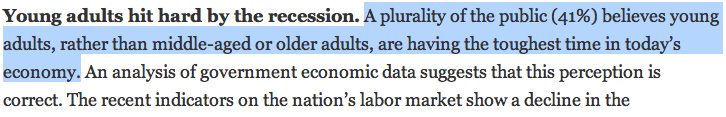
\includegraphics[width=0.95\textwidth]{4-1_var_in_est/figures/pew/pew2} \\
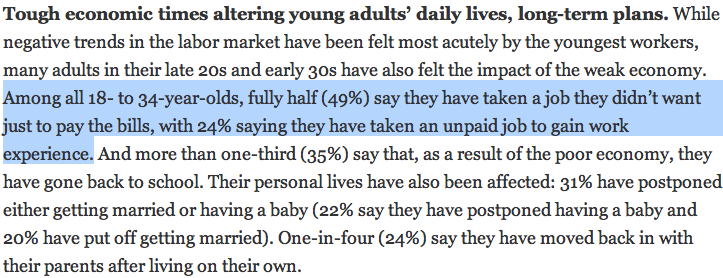
\includegraphics[width=0.95\textwidth]{4-1_var_in_est/figures/pew/pew3}
\end{center}

\ct{\webURL{http://pewresearch.org/pubs/2191/young-adults-workers-labor-market-pay-careers-advancement-recession}}

\end{frame}

%%%%%%%%%%%%%%%%%%%%%%%%%%%%%%%%%%%%

\begin{frame}
\frametitle{Margin of error}

\begin{center}
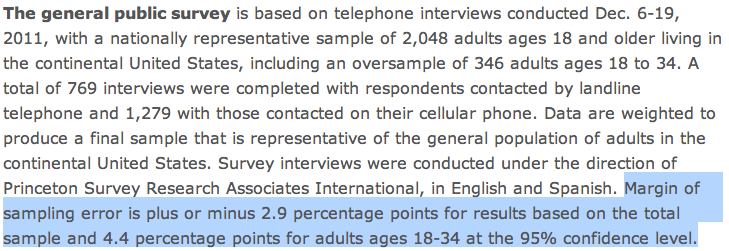
\includegraphics[width=0.95\textwidth]{4-1_var_in_est/figures/pew/pew4}
\end{center}

\begin{itemize}

\item 41\% $\pm$ 2.9\%: We are 95\% confident that 38.1\% to 43.9\% of the public believe young adults, rather than middle-aged or older adults, are having the toughest time in today's economy.


\item 49\% $\pm$ 4.4\%: We are 95\% confident that 44.6\% to 53.4\% of 18-34 years olds have taken a job they didn't want just to pay the bills.

\end{itemize}

\end{frame}

%%%%%%%%%%%%%%%%%%%%%%%%%%%%%%%%%%%%

\begin{frame}
\frametitle{Parameter estimation}

\begin{itemize}

\item We are often interested in \hl{population parameters}.

\item Since complete populations are difficult (or impossible) to collect data on, we use \hl{sample statistics} as \hl{point estimates} for the unknown population parameters of interest.

\item Sample statistics vary from sample to sample.

\item Quantifying how sample statistics vary provides a way to estimate the \hl{margin of error} associated with our point estimate.

\item But before we get to quantifying the variability among samples, let's try to understand how and why point estimates vary from sample to sample.

\end{itemize}

\dq{Suppose we randomly sample 1,000 adults from each state in the US. Would
you expect the sample means of their heights to be the same, somewhat different, or very different?}

\pause

\soln{Not the same, but only somewhat different.}

\end{frame}

%%%%%%%%%%%%%%%%%%%%%%%%%%%%%%%%%%%

\subsection{Application exercise}

%%%%%%%%%%%%%%%%%%%%%%%%%%%%%%%%%%%

\begin{frame}
\frametitle{}

\dq{The following histogram shows the distribution of number of drinks it takes a group of college students to get drunk. We will assume that this is our population of interest. If we randomly select observations from this data set, which values are most likely to be selected, which are least likely?}

\begin{center}
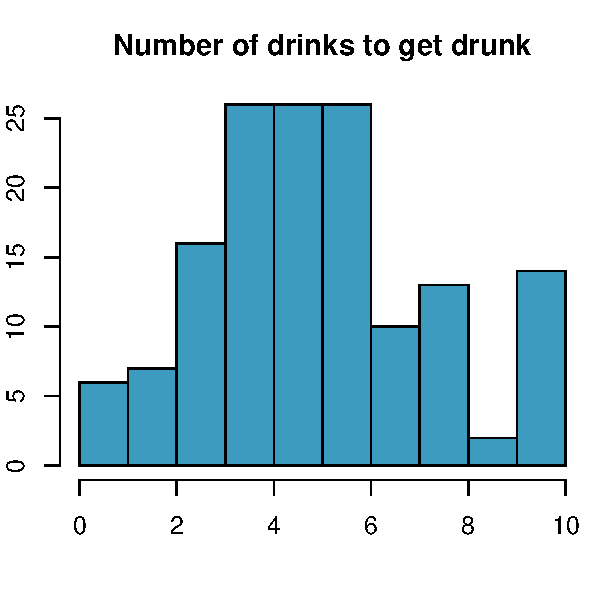
\includegraphics[width=0.5\textwidth]{4-1_var_in_est/figures/no_drinks_drunk/no_drinks_drunk} 
\end{center}

\end{frame}

%%%%%%%%%%%%%%%%%%%%%%%%%%%%%%%%%%

\begin{frame}[fragile]
\frametitle{}

\vspace{-0.25cm}

\dq{Suppose that you don't have access to the population data. In order to estimate the average number of drinks it takes these college students to get drunk, you might sample from the population and use your sample mean as the best guess for the unknown population mean.

\begin{itemize}

\item Sample, with replacement, ten students from the population, and record the number of drinks it takes them to get drunk.

\item Find the sample mean.

\item Plot the distribution of the sample averages  obtained by members of the class.

\end{itemize}
}

\vspace{-0.25cm}

\begin{center}
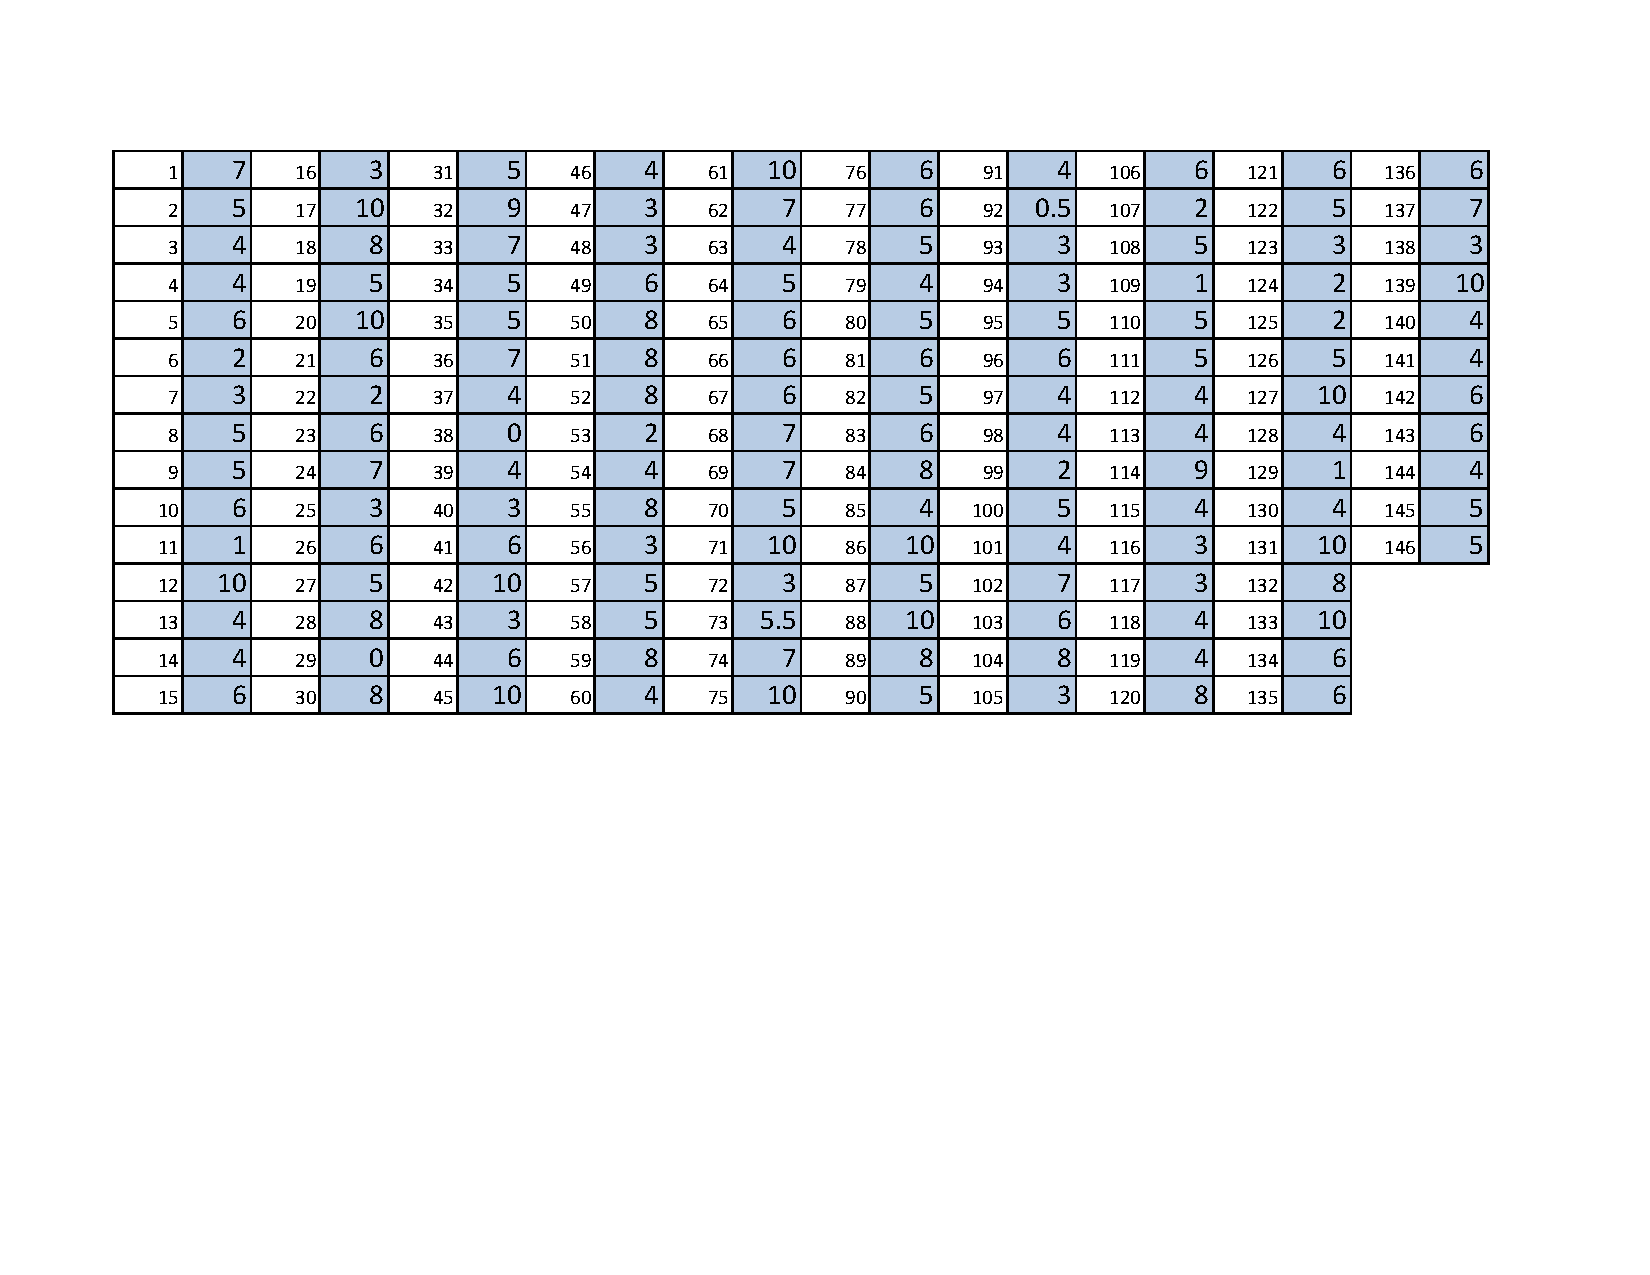
\includegraphics[width=0.8\textwidth]{4-1_var_in_est/figures/no_drinks_drunk/no_drinks_drunk_clean} 
\end{center}

\end{frame}

%%%%%%%%%%%%%%%%%%%%%%%%%%%%%%%%%%%

\begin{frame}[fragile]
\frametitle{}

\dq{Example:} List of random numbers: 59, 121,  88,  46,  58,  72,  82,  81,   5,  10 \\

\begin{center}
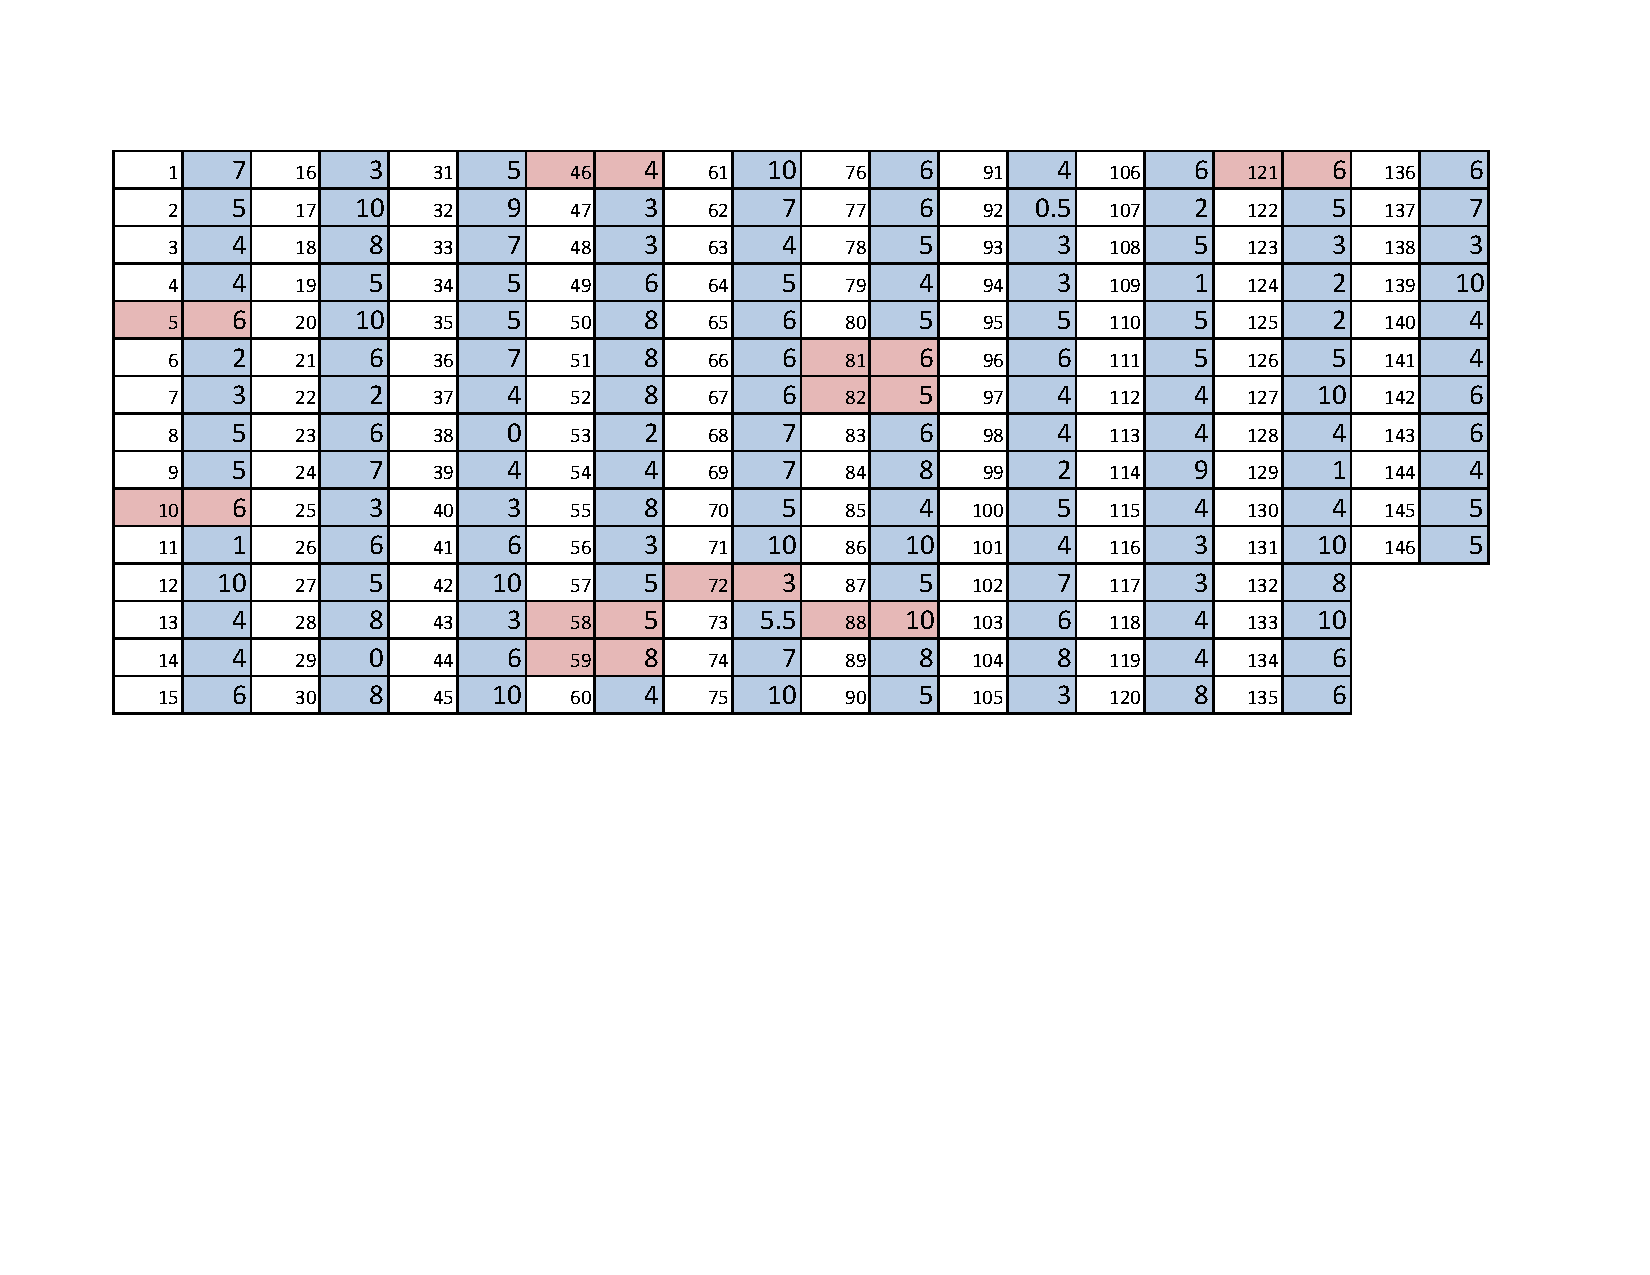
\includegraphics[width=0.9\textwidth]{4-1_var_in_est/figures/no_drinks_drunk/no_drinks_drunk_marked} 
\end{center}

\pause

Sample mean: (8+6+10+4+5+3+5+6+6+6) / 10 = 5.9

\end{frame}

%%%%%%%%%%%%%%%%%%%%%%%%%%%%%%%%%


\begin{frame}[fragile]
\frametitle{Sampling distribution}

What you just constructed is called a \hl{sampling distribution}.

\pause

$\:$ \\
\dq
{What is the shape and center of this distribution? Based on this distribution, what do you think is the true population average?}

$\:$ \\
\soln{\only<3>{
Approximately 5.39, the true population mean.
}}

\end{frame}


%%%%%%%%%%%%%%%%%%%%%%%%%%%%%%%%%%

\subsection{Sampling distributions - via CLT}

%%%%%%%%%%%%%%%%%%%%%%%%%%%%%%%%%%

\begin{frame}
\frametitle{Central limit theorem}

\formula{Central limit theorem}
{The distribution of the sample mean is well approximated by a normal model:
\[ \bar{x} \sim N \pr{ mean = \mu, SE = \frac{\sigma}{\sqrt{n}} }, \]
where SE is represents \hl{standard error}, which is defined as the standard deviation of the sampling distribution. If $\sigma$ is unknown, use $s$.
}

\begin{itemize}

\item It wasn't a coincidence that the sampling distribution we saw earlier was symmetric, and centered at the true population mean.

\item We won't go through a detailed proof of why $SE =  \frac{\sigma}{\sqrt{n}}$, but note that as $n$ increases $SE$ decreases. 
\begin{itemize}
\item As the sample size increases we would expect samples to yield more consistent sample means, hence the variability among the sample means would be lower.
\end{itemize}

\end{itemize}

\end{frame}

%%%%%%%%%%%%%%%%%%%%%%%%%%%%%%%%%%%%

\begin{frame}
\frametitle{CLT - conditions}

Certain conditions must be met for the CLT to apply:

\begin{enumerate}

\item \hlGr{Independence:} Sampled observations must be independent. \\

This is difficult to verify, but is more likely if
\begin{itemize}
\item random sampling/assignment is used, and
\item if sampling without replacement, $n$ $<$ 10\% of the population.
\end{itemize}

\pause

\item \hlGr{Sample size/skew:} Either the population distribution is normal, or if the population distribution is skewed, the sample size is large.\\
\begin{itemize}
\item the more skewed the population distribution, the larger sample size we need for the CLT to apply
\item for moderately skewed distributions $n>30$ is a widely used rule of thumb \\
\end{itemize}

This is also difficult to verify for the population, but we can check it using the sample data, and assume that the sample mirrors the population.

\end{enumerate}

\end{frame}

%%%%%%%%%%%%%%%%%%%%%%%%%%%%%%%%%%%%
%%%%%%%%%%%%%%%%%%%%%%%%%%%%%%%%%%%%

\section{Confidence intervals}

%%%%%%%%%%%%%%%%%%%%%%%%%%%%%%%%%%%%

\subsection{Why do we report confidence intervals?}

%%%%%%%%%%%%%%%%%%%%%%%%%%%%%%%%%%%%

\begin{frame}[shrink]
\frametitle{Confidence intervals}

\begin{itemize}

\item A plausible range of values for the population parameter is called a \hl{confidence interval}.

\item Using only a sample statistic to estimate a parameter is like fishing in a murky lake with a spear, and using a confidence interval is like fishing with a net.
$\:$ \\
$\:$ \\
\begin{columns}[c]
\column{0.25\textwidth}
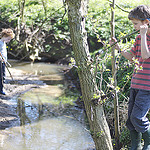
\includegraphics[width=\textwidth]{4-2_conf_int/figures/spear}
\column{0.5\textwidth}
{\small
We can throw a spear where we saw a fish but we will probably miss. If we toss a net in that area, we have a good chance of catching the fish.
}
\column{0.25\textwidth}
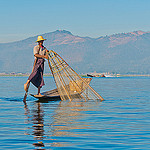
\includegraphics[width=\textwidth]{4-2_conf_int/figures/net}
\end{columns}
$\:$ \\
\item If we report a point estimate, we probably won't hit the exact population parameter. If we report a range of plausible values we have a good shot at capturing the parameter. 

\end{itemize}

{\tiny Photos by Mark Fischer (http://www.flickr.com/photos/fischerfotos/7439791462) and Chris Penny (http://www.flickr.com/photos/clearlydived/7029109617) on Flickr.}

% spear fig: http://www.flickr.com/photos/clearlydived/7029109617/sizes/q/
% net fig: http://www.flickr.com/photos/fischerfotos/7439791462/sizes/q/

\end{frame}

%%%%%%%%%%%%%%%%%%%%%%%%%%%%%%%%%%%%

\subsection{Constructing a confidence interval}

%%%%%%%%%%%%%%%%%%%%%%%%%%%%%%%%%%%%

\begin{frame}
\frametitle{Average number of exclusive relationships}

\dq{A random sample of 50 college students were asked how many exclusive relationships they have been in so far. This sample yielded a mean of 3.2 and a standard deviation of 1.74. Estimate the true average number of exclusive relationships using this sample.}

\pause 

\vspace{-0.5cm}
\[ \bar{x} = 3.2 \qquad s = 1.74 \]

\pause

The approximate 95\% confidence interval is defined as 
\[ point~estimate \pm 2 \times SE \]

\pause

\vspace{-0.25cm}
\[ SE = \frac{s}{\sqrt{n}} = \frac{1.74}{\sqrt{50}} \approx 0.25 \]

\pause

\vspace{-0.25cm}
\begin{eqnarray*}
\bar{x} \pm 2 \times SE &=& 3.2 \pm 2 \times 0.25 \\
\pause
&=& (3.2 - 0.5, 3.2 + 0.5) \\
\pause
&=& (2.7, 3.7)
\end{eqnarray*}


\end{frame}

%%%%%%%%%%%%%%%%%%%%%%%%%%%%%%%%%%%

\begin{frame}
\frametitle{}

\pq{Which of the following is the correct interpretation of this confidence interval?}

We are 95\% confident that
\begin{enumerate}[(a)]
\item the average number of exclusive relationships college students in this sample have been in is between 2.7 and 3.7.
\solnMult{college students on average have been in between 2.7 and 3.7 exclusive relationships.}
\item a randomly chosen college student has been in 2.7 to 3.7 exclusive relationships.
\item 95\% of college students have been in 2.7 to 3.7 exclusive relationships.
\end{enumerate}

\end{frame}

%%%%%%%%%%%%%%%%%%%%%%%%%%%%%%%%%%%

\subsection{A more accurate interval}

%%%%%%%%%%%%%%%%%%%%%%%%%%%%%%%%%%%

\begin{frame}
\frametitle{A more accurate interval}

\formula{Confidence interval, a general formula}
{\[ point~estimate\pm z^\star \times SE \] }

\pause

Conditions when the point estimate = $\bar{x}$:
\begin{enumerate}

\item \hlGr{Independence:} Observations in the sample must be independent
\begin{itemize}
\item random sample/assignment
\item if sampling without replacement, $n <$ 10\% of population
\end{itemize}

\item \hlGr{Sample size / skew:} $n \ge 30$ and population distribution should not be extremely skewed

\end{enumerate}

$\:$ \\
\pause

\orange{Note:} We will discuss working with samples where $n < 30$ in the next chapter.

\end{frame}

%%%%%%%%%%%%%%%%%%%%%%%%%%%%%%%%%%%%

\subsection{Capturing the population parameter}

%%%%%%%%%%%%%%%%%%%%%%%%%%%%%%%%%%%

\begin{frame}
\frametitle{What does 95\% confident mean?}

\begin{itemize}

\item Suppose we took many samples and built a confidence interval from each sample using the equation $point~estimate \pm 2 \times SE$.

\item Then about 95\% of those intervals would contain the true population mean ($\mu$). 

\end{itemize}

\twocol{0.5}{0.5}
{
\begin{itemize}

\item The figure shows this process with 25 samples, where 24 of the resulting confidence intervals contain the true average number of exclusive relationships, and one does not.

\end{itemize}
}
{
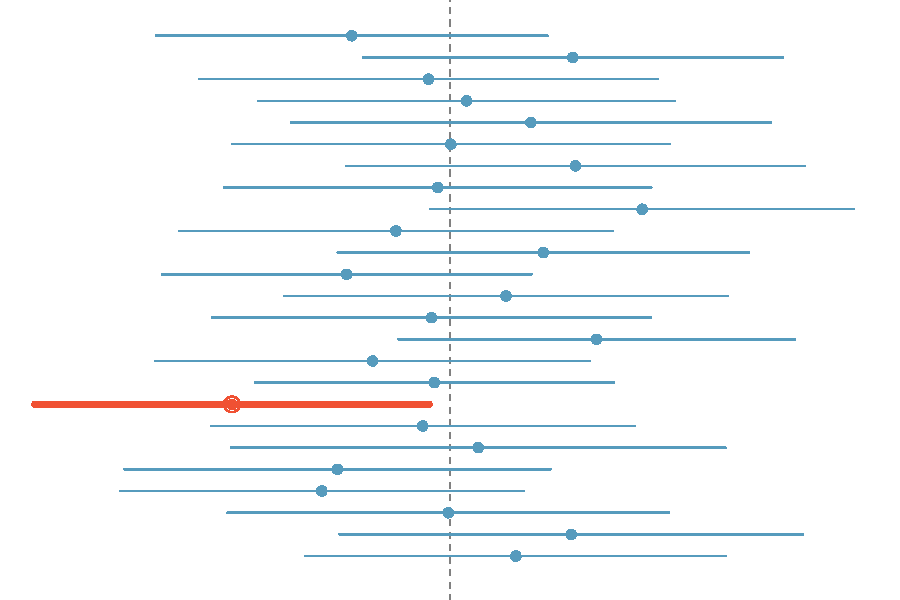
\includegraphics[width=\textwidth]{4-2_conf_int/figures/95PercentConfidenceInterval/95PercentConfidenceInterval}
}

\end{frame}

%%%%%%%%%%%%%%%%%%%%%%%%%%%%%%%%%%%

\begin{frame}
\frametitle{Width of an interval}

\dq{If we want to be more certain that we capture the population parameter, i.e. increase our confidence level, should we use a wider interval or a smaller interval?}

\pause

\soln{A wider interval.}

$\:$ \\

\pause

\dq{Can you see any drawbacks to using a wider interval?}
\begin{center}

\includegraphics[width=0.9\textwidth]{4-2_conf_int/figures/garfield}
\end{center}

\pause

\soln{If the interval is too wide it may not be very informative.}

\end{frame}

{\scriptsize Image source: http://web.as.uky.edu/statistics/users/earo227/misc/garfield\_weather.gif}

%%%%%%%%%%%%%%%%%%%%%%%%%%%%%%%%%%%

\subsection{Changing the confidence level}

%%%%%%%%%%%%%%%%%%%%%%%%%%%%%%%%%%%

\begin{frame}
\frametitle{Changing the confidence level}

\[ point~estimate\pm z^\star \times SE \] 

\begin{itemize}

\item In a confidence interval, $z^\star \times SE$ is called the \hl{margin of error}, and for a given sample, the margin of error changes as the confidence level changes.

\item In order to change the confidence level we need to adjust $z^\star$ in the above formula.

\item Commonly used confidence levels in practice are 90\%, 95\%, 98\%, and 99\%.

\item For a 95\% confidence interval, $z^\star = 1.96$.

\item However, using the standard normal ($z$) distribution, it is possible to find the appropriate $z^\star$ for any confidence level.

\end{itemize}

\end{frame}

%%%%%%%%%%%%%%%%%%%%%%%%%%%%%%%%%%%%

\begin{frame}

\pq{Which of the below Z scores is the appropriate $z^\star$ when calculating a 98\% confidence interval?}

\begin{multicols}{2}
\begin{enumerate}[(a)]
\item $Z = 2.05$
\item $Z = 1.96$
\solnMult{$Z = 2.33$}
\item $Z = -2.33$
\item $Z = -1.65$
\item[]
\end{enumerate}
\end{multicols}

\soln{\only<2>{
\begin{center}
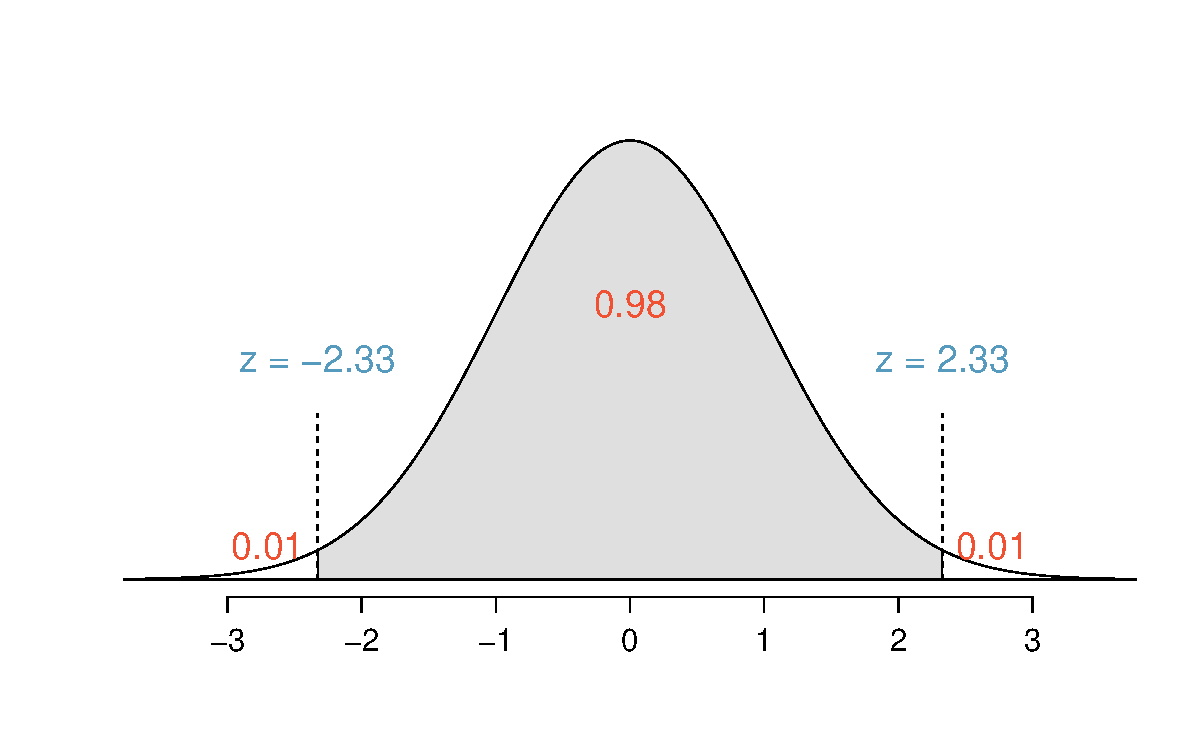
\includegraphics[width=0.7\textwidth]{4-2_conf_int/figures/middle98/middle98}
\end{center}
}}

\end{frame}

%%%%%%%%%%%%%%%%%%%%%%%%%%%%%%%%%%%

%%%%%%%%%%%%%%%%%%%%%%%%%%%%%%%%%%%%

\section{Hypothesis testing}

%%%%%%%%%%%%%%%%%%%%%%%%%%%%%%%%%%%%

\subsection{Hypothesis testing framework}

%%%%%%%%%%%%%%%%%%%%%%%%%%%%%%%%%%%%

\begin{frame}
\frametitle{Remember when...}

Gender discrimination experiment:

{\small
\begin{tabular}{ll  cc c} 
  		&				& \multicolumn{2}{c}{\textit{Promotion}} \\
\cline{3-4}
							&			& Promoted	& Not Promoted 	& Total	\\
\cline{2-5}
\multirow{2}{*}{\textit{Gender	}}	&Male 		& 21	 	& 3		& 24 	\\
							&Female		& 14	 	& 10 	 	& 24 \\
\cline{2-5}
							&Total		& 35		& 13		& 48 \\
\end{tabular}
}

\pause

\[ \hat{p}_{males} = 21 / 24 \approx 0.88 \]
\[ \hat{p}_{females} = 14 / 24 \approx 0.58 \]

\pause

Possible explanations:
\begin{itemize}
\item Promotion and gender are \hl{independent}, no gender discrimination, observed difference in proportions is simply due to chance. $\rightarrow$ \red{null} - {\small (nothing is going on)}
\item Promotion and gender are \hl{dependent}, there is gender discrimination, observed difference in proportions is not due to chance. $\rightarrow$ \red{alternative} - {\small (something is going on)}

\end{itemize}

\end{frame}

%%%%%%%%%%%%%%%%%%%%%%%%%%%%%%%%%%%%

\begin{frame}
\frametitle{Result}

\begin{center}
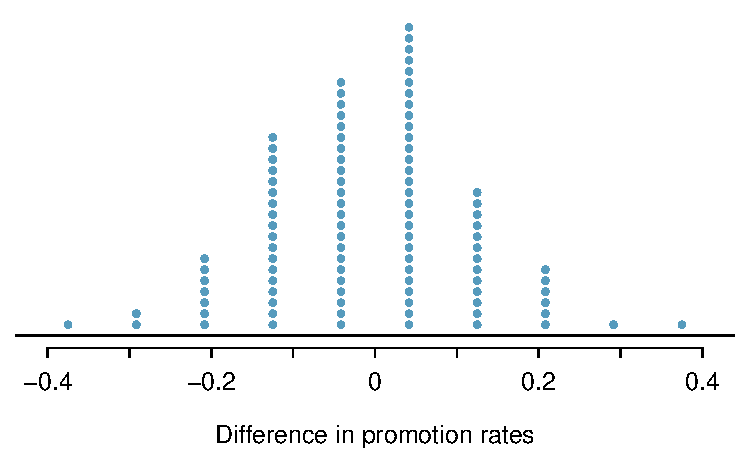
\includegraphics[width=0.75\textwidth]{4-3_hyp_test/figures/discRandDotPlot/discRandDotPlot}
\end{center}

\pause

Since it was quite unlikely to obtain results like the actual data or something more extreme in the simulations (male promotions being 30\% or more higher than female promotions), we decided to reject the null hypothesis in favor of the alternative.

\end{frame}

%%%%%%%%%%%%%%%%%%%%%%%%%%%%%%%%%%%%

\begin{frame}
\frametitle{Recap: hypothesis testing framework}

\begin{itemize}
\item We start with a \hl{null hypothesis ($H_0$)} that represents the status quo.
\pause
\item We also have an \hl{alternative hypothesis ($H_A$)} that represents our research question, i.e. what we're testing for.
\pause
\item We conduct a hypothesis test under the assumption that the null hypothesis is true, either via simulation or traditional methods based on the central limit theorem (coming up next...).
\pause
\item If the test results suggest that the data do not provide convincing evidence for the alternative hypothesis, we stick with the null hypothesis. If they do, then we reject the null hypothesis in favor of the alternative.
\end{itemize}
\pause
We'll formally introduce the hypothesis testing framework using an example on testing a claim about a population mean.

\end{frame}

%%%%%%%%%%%%%%%%%%%%%%%%%%%%%%%%%%%%

\subsection{Testing hypotheses using confidence intervals} 

%%%%%%%%%%%%%%%%%%%%%%%%%%%%%%%%%%%%

\begin{frame}
\frametitle{Testing hypotheses using confidence intervals}

\dq{Earlier we calculated a 95\% confidence interval for the average number of exclusive relationships college students have been in to be (2.7, 3.7). Based on this confidence interval, do these data support the hypothesis that college students on average have been in more than 3 exclusive relationships.}

\pause

\begin{itemize}

\item The associated hypotheses are:
\begin{itemize}
\item[$H_0$:] $\mu = 3$: College students have been in 3 exclusive relationships, on average
\item[$H_A$:] $\mu > 3$: College students have been in more than 3 exclusive relationships, on average
\end{itemize}

\pause

\item Since the null value is included in the interval, we do not reject the null hypothesis in favor of the alternative.

\pause

\item This is a quick-and-dirty approach for hypothesis testing. However it doesn't tell us the likelihood of certain outcomes under the null hypothesis, i.e. the p-value, based on which we can make a decision on the hypotheses.

\end{itemize}

\end{frame}

%%%%%%%%%%%%%%%%%%%%%%%%%%%%%%%%%%%%

\begin{frame}
\frametitle{Number of college applications}

\dq{{\small A similar survey asked how many colleges students applied to, and 206 students responded to this question. This sample yielded an average of 9.7 college applications with a standard deviation of 7. College Board website states that counselors recommend students apply to roughly 8 colleges.  Do these data provide convincing evidence that the average number of colleges all Duke students apply to is \emph{higher} than recommended?}}

\vfill

\ct{\webURL{http://www.collegeboard.com/student/apply/the-application/151680.html}}

\end{frame}

%%%%%%%%%%%%%%%%%%%%%%%%%%%%%%%%%%

\begin{frame}
\frametitle{Setting the hypotheses}

\begin{itemize}

\item The \hl{parameter of interest} is the average number of schools applied to by \underline{all} Duke students.

\pause

\item There may be two explanations why our sample mean is higher than the recommended 8 schools.
\begin{itemize}
\item The true population mean is different.
\item The true population mean is 8, and the difference between the true population mean and the sample mean is simply due to natural sampling variability.
\end{itemize}

\pause

\item We start with the assumption the average number of colleges Duke students apply to is 8 (as recommended)
\[ \mathhl{H_0:}~\mu = 8 \]

\pause

\item We test the claim that the average number of colleges Duke students apply to is greater than 8
\[ \mathhl{H_A:}~\mu > 8 \]

\end{itemize}

\end{frame}

%%%%%%%%%%%%%%%%%%%%%%%%%%%%%%%%%%%

\subsection{Conditions for inference}

%%%%%%%%%%%%%%%%%%%%%%%%%%%%%%%%%%%

\begin{frame}
\frametitle{Number of college applications - conditions}

\pq{Which of the following is \emph{not} a condition that needs to be met to proceed with this hypothesis test?}

\begin{enumerate}[(a)]
\item Students in the sample should be independent of each other with respect to how many colleges they applied to.
\item Sampling should have been done randomly.
\item The sample size should be less than 10\% of the population of all Duke students.
\solnMult{ There should be at least 10 successes and 10 failures in the sample.}
\item The distribution of the number of colleges students apply to should not be extremely skewed.
\end{enumerate}

\end{frame}

%%%%%%%%%%%%%%%%%%%%%%%%%%%%%%%%%%

\subsection{Formal testing using p-values}

%%%%%%%%%%%%%%%%%%%%%%%%%%%%%%%%%%%%

\begin{frame}
\frametitle{Test statistic}

In order to evaluate if the observed sample mean is unusual for the hypothesized sampling distribution, we determine how many standard errors away from the null it is, which is also called the \hl{test statistic}.

\pause

\twocol{0.55}{0.45}{
\begin{center}
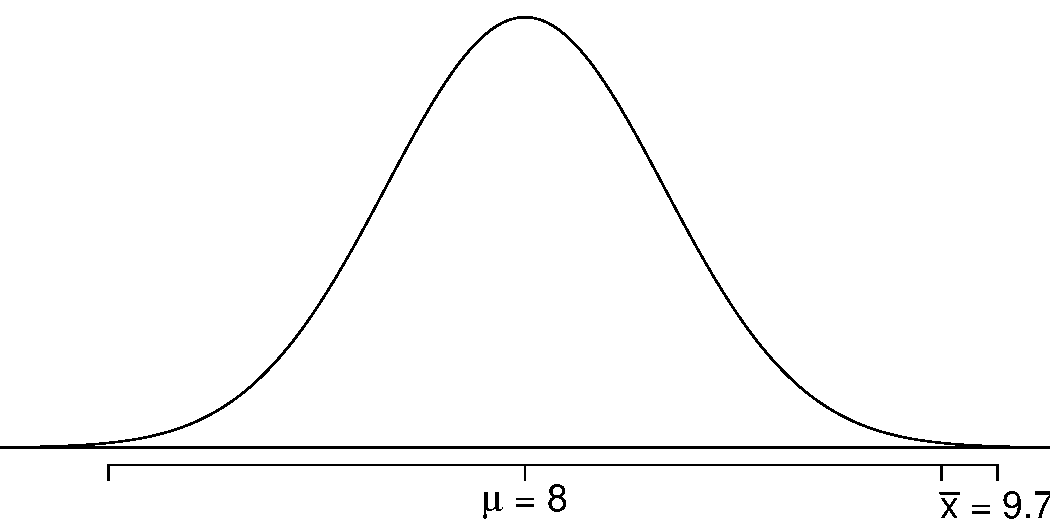
\includegraphics[width=\textwidth]{4-3_hyp_test/figures/app/app_z}
\end{center}
\pause
\[ \bar{x} \sim N \pr{ \mu = 8, SE = \frac{7}{\sqrt{206}} = 0.5 } \]
\pause
\[ Z = \frac{9.7 - 8}{0.5} = 3.4 \]
}
{
\pause
\dq{The sample mean is 3.4 standard errors away from the hypothesized value. Is this considered unusually high? That is, is the result \hl{statistically significant}?}
\pause
\soln{Yes, and we can quantify how unusual it is using a p-value.}
}

\end{frame}

%%%%%%%%%%%%%%%%%%%%%%%%%%%%%%%%%%%

\begin{frame}
\frametitle{p-values}

\begin{itemize}

\item We then use this test statistic to calculate the \hl{p-value}, the probability of observing data at least as favorable to the alternative hypothesis as our current data set, if the null hypothesis were true.

\pause

\item If the p-value is \hl{low} (lower than the significance level, $\alpha$, which is usually 5\%) we say that it would be very unlikely to observe the data if the null hypothesis were true, and hence \hl{reject $H_0$}.

\pause

\item If the p-value is \hl{high} (higher than $\alpha$) we say that it is likely to observe the data even if the null hypothesis were true, and hence \hl{do not reject $H_0$}.

\end{itemize}

\end{frame}

%%%%%%%%%%%%%%%%%%%%%%%%%%%%%%%%%%%%

\begin{frame}
\frametitle{Number of college applications - p-value}

\hl{p-value:} probability of observing data at least as favorable to $H_A$ as our current data set (a sample mean greater than 9.7), if in fact $H_0$ were true (the true population mean was 8).

\begin{center}
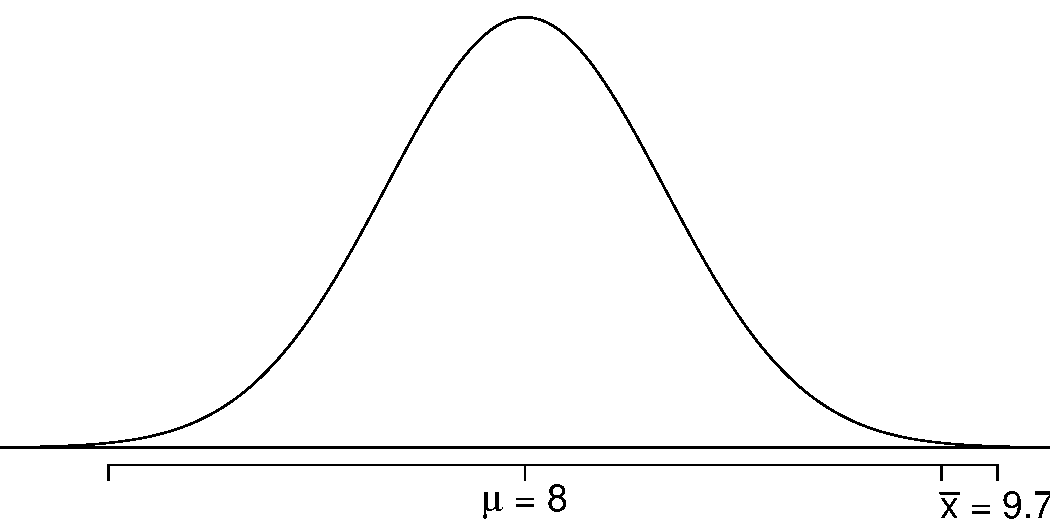
\includegraphics[width=0.55\textwidth]{4-3_hyp_test/figures/app/app_pval_gr}
\end{center}

\pause

\[ P(\bar{x} > 9.7~|~\mu = 8) = P(Z > 3.4) = 0.0003 \]

\end{frame}

%%%%%%%%%%%%%%%%%%%%%%%%%%%%%%%%%%

\begin{frame}
\frametitle{Number of college applications - Making a decision}

\begin{itemize}

\item p-value = 0.0003

\pause

\begin{itemize}
\item If the true average of the number of colleges Duke students applied to is 8, there is only 0.03\% chance of observing a random sample of 206 Duke students who on average apply to 9.7 or more schools.
\pause
\item This is a pretty low probability for us to think that a sample mean of 9.7 or more schools is likely to happen simply by chance.
\end{itemize}

\pause
\item Since p-value is \red{low} (lower than 5\%) we \red{reject $H_0$}.

\pause
\item The data provide convincing evidence that Duke students apply to more than 8 schools on average.

\pause
\item The difference between the null value of 8 schools and observed sample mean of 9.7 schools is \red{not due to chance} or sampling variability.

\end{itemize}

\end{frame}

%%%%%%%%%%%%%%%%%%%%%%%%%%%%%%%%%%%%

\begin{frame}
\frametitle{}

\pq{{\footnotesize A poll by the National Sleep Foundation found that college students average about 7 hours of sleep per night. A sample of 169 college students taking an introductory statistics class yielded an average of 6.88 hours, with a standard deviation of  0.94 hours. Assuming that this is a random sample representative of all college students {\scriptsize \textit{(bit of a leap of faith?)}}, a hypothesis test was conducted to evaluate if college students on average sleep \emph{less than} 7 hours per night. The p-value for this hypothesis test is 0.0485. Which of the following is correct?}}

\begin{enumerate}[(a)]
\item Fail to reject $H_0$, the data provide convincing evidence that college students sleep less than 7 hours on average.
\solnMult{ Reject $H_0$, the data provide convincing evidence that college students sleep less than 7 hours on average. }
\item Reject $H_0$, the data prove that college students sleep more than 7 hours on average.
\item Fail to reject $H_0$, the data do not provide convincing evidence that college students sleep less than 7 hours on average.
\item Reject $H_0$, the data provide convincing evidence that college students in this sample sleep less than 7 hours on average.
\end{enumerate}

\end{frame}

%%%%%%%%%%%%%%%%%%%%%%%%%%%%%%%%%

\subsection{Two-sided hypothesis testing with p-values}

%%%%%%%%%%%%%%%%%%%%%%%%%%%%%%%%%

\begin{frame}
\frametitle{Two-sided hypothesis testing with p-values}

\begin{itemize}

\item If the research question was ``Do the data provide convincing evidence that the average amount of sleep college students get per night is \red{different} than the national average?", the alternative hypothesis would be different.
\begin{align*}
H_0&: \mu = 7 \\
H_A&: \mu \red{~$\ne$~} 7
\end{align*}

\pause

\item Hence the p-value would change as well:
\twocol{0.55}{0.45}
{
\begin{center}
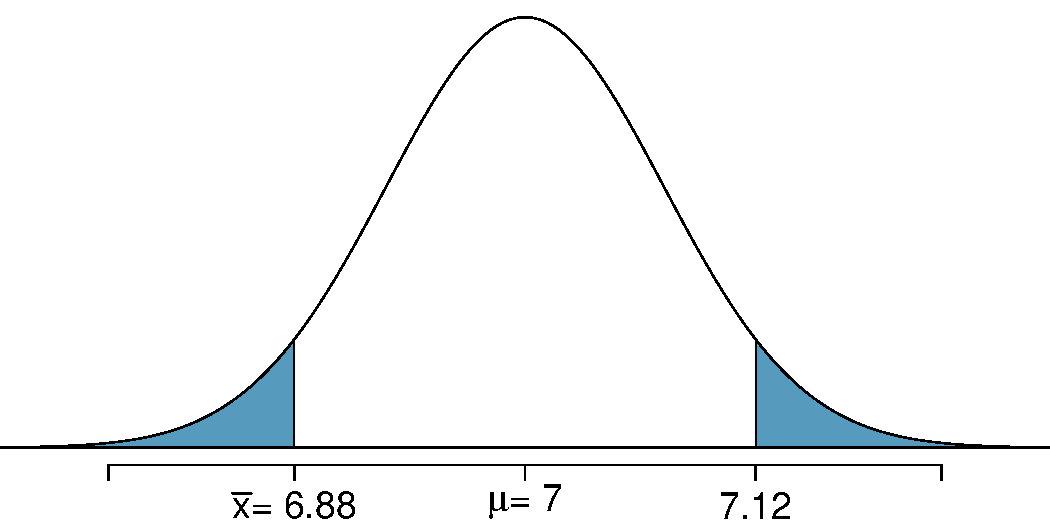
\includegraphics[width=\textwidth]{4-3_hyp_test/figures/sleep/sleep_pval_ts}
\end{center}
}
{
p-value \\
$= 0.0485 \times 2$ \\
$= 0.097$
}

\end{itemize}

\end{frame}

%%%%%%%%%%%%%%%%%%%%%%%%%%%%%%%%%%%%

\subsection{Decision errors}

%%%%%%%%%%%%%%%%%%%%%%%%%%%%%%%%%%%%

\begin{frame}
\frametitle{Decision errors}

\begin{itemize}

\item Hypothesis tests are not flawless.

\item In the court system innocent people are sometimes wrongly convicted and the guilty sometimes walk free.

\item Similarly, we can make a wrong decision in statistical hypothesis tests as well. 

\item The difference is that we have the tools necessary to quantify how often we make errors in statistics.

\end{itemize}

\end{frame}

%%%%%%%%%%%%%%%%%%%%%%%%%%%%%%%%%%%%

\begin{frame}
\frametitle{Decision errors (cont.)}

There are two competing hypotheses: the null and the alternative. In a hypothesis test, we make a decision about which might be true, but our choice might be incorrect. \\

\pause

\begin{center}
\begin{tabular}{l l | c c}
\multicolumn{2}{c}{} & \multicolumn{2}{c}{\textbf{Decision}} \\
& & fail to reject $H_0$ &  reject $H_0$ \\
  \cline{2-4}
& $H_0$ true & \onslide<3->{\green{$\checkmark$}} &  \onslide<5->{\red{Type 1 Error}} \\
\raisebox{1.5ex}{\textbf{Truth}} & $H_A$ true & \onslide<6->{\red{Type 2 Error}} & \onslide<4->{\green{$\checkmark$}} \\
  \cline{2-4}
\end{tabular}
\end{center}

\begin{itemize}
\item \onslide<5->{A \hl{Type 1 Error} is rejecting the null hypothesis when $H_0$ is true.}

\item \onslide<6->{A \hl{Type 2 Error} is failing to reject the null hypothesis when $H_A$ is true.}

\item \onslide<7->{We (almost) never know if $H_0$ or $H_A$ is true, but we need to consider all possibilities.}

\end{itemize}

\end{frame}

%%%%%%%%%%%%%%%%%%%%%%%%%%%%%%%%%%%%

\begin{frame}
\frametitle{Hypothesis Test as a trial}

If we again think of a hypothesis test as a criminal trial then it makes sense to frame the verdict in terms of the null and alternative hypotheses:
\begin{align*}
H_0&:\text{ Defendant is innocent} \\
H_A&:\text{ Defendant is guilty}
\end{align*}

Which type of error is being committed in the following circumstances?

\begin{itemize}
\item Declaring the defendant innocent when they are actually guilty
\soln{\only<2->{\begin{center}\hl{Type 2 error}\end{center}}}
\item Declaring the defendant guilty when they are actually innocent
\soln{\only<3->{\begin{center}\hl{Type 1 error}\end{center}}}
\end{itemize}

\only<4->{Which error do you think is the worse error to make?}
\only<5>{\begin{center}{\footnotesize ``better that ten guilty persons escape than that one innocent suffer''\\ -- William Blackstone}\end{center}}
\end{frame}

%%%%%%%%%%%%%%%%%%%%%%%%%%%%%%%%%%%%

\begin{frame}
\frametitle{Type 1 error rate}

\begin{itemize}

\item As a general rule we reject $H_0$ when the p-value is less than 0.05, i.e. we use a \hl{significance level} of 0.05, \mathhl{\alpha = 0.05}.

\pause

\item This means that, for those cases where $H_0$ is actually true, we do not want to incorrectly reject it more than 5\% of those times. 

\pause

\item In other words, when using a 5\% significance level there is about 5\% chance of making a Type 1 error if the null hypothesis is true.
\[ \mathhl{ P(\text{Type 1 error | $H_0$ true}) = \alpha } \]

\pause

\item This is why we prefer small values of $\alpha$ -- increasing $\alpha$ increases the Type 1 error rate.

\end{itemize}

\end{frame}

%%%%%%%%%%%%%%%%%%%%%%%%%%%%%%%%%%%%

\subsection{Choosing a significance level}

%%%%%%%%%%%%%%%%%%%%%%%%%%%%%%%%%%%%

\begin{frame}
\frametitle{Choosing a significance level}

\begin{itemize}

\item Choosing a significance level for a test is important in many contexts, and the traditional level is 0.05. However, it is often helpful to adjust the significance level based on the application. 

\item We may select a level that is smaller or larger than 0.05 depending on the consequences of any conclusions reached from the test.

\item If making a Type 1 Error is dangerous or especially costly, we should choose a small significance level (e.g. 0.01). Under this scenario we want to be very cautious about rejecting the null hypothesis, so we demand very strong evidence favoring $H_A$ before we would reject $H_0$.

\item If a Type 2 Error is relatively more dangerous or much more costly than a Type 1 Error, then we should choose a higher significance level (e.g. 0.10). Here we want to be cautious about failing to reject $H_0$ when the null is actually false.

\end{itemize}

\end{frame}

%%%%%%%%%%%%%%%%%%%%%%%%%%%%%%%%%%%%

\subsection{Recap}

%%%%%%%%%%%%%%%%%%%%%%%%%%%%%%%%%%%%

\begin{frame}

\vfill

\textit{the next two slides are provided as a brief summary of hypothesis testing...}

\vfill

\end{frame}

%%%%%%%%%%%%%%%%%%%%%%%%%%%%%%%%%%%%

\begin{frame}
\frametitle{Recap: Hypothesis testing framework}

\begin{enumerate}

\item Set the hypotheses.

\item Check assumptions and conditions.

\item Calculate a \hl{test statistic} and a p-value.

\item Make a decision, and interpret it in context of the research question.

\end{enumerate}

\end{frame}

%%%%%%%%%%%%%%%%%%%%%%%%%%%%%%%%%%%

\begin{frame}
\frametitle{Recap: Hypothesis testing for a population mean}

\begin{enumerate}

\item Set the hypotheses
\begin{itemize}
\item $H_0: \mu = null~value$
\item $H_A: \mu <$ or $>$ or $\ne null~value$
\end{itemize}

\item Calculate the point estimate

\item Check assumptions and conditions
\begin{itemize}
\item Independence: random sample/assignment, 10\% condition when sampling without replacement
\item Normality: nearly normal population or $n \ge 30$, no extreme skew -- or use the t distribution
\end{itemize}

\item Calculate a \hl{test statistic} and a p-value (draw a picture!)
\[ Z = \frac{\bar{x} - \mu}{SE},~where~SE = \frac{s}{\sqrt{n}} \]

\item Make a decision, and interpret it in context
\begin{itemize}
\item If p-value $< \alpha$, reject $H_0$, data provide evidence for $H_A$
\item If p-value $> \alpha$, do not reject $H_0$, data do not provide evidence for $H_A$
\end{itemize}

\end{enumerate}

\end{frame}

%%%%%%%%%%%%%%%%%%%%%%%%%%%%%%%%%%%%
%%%%%%%%%%%%%%%%%%%%%%%%%%%%%%%%%%%

\section{Examining the Central Limit Theorem}

%%%%%%%%%%%%%%%%%%%%%%%%%%%%%%%%%%%

\begin{frame}[fragile]
\frametitle{Average number of basketball games attended}

Next let's look at the population data for the number of basketball games attended:

\begin{center}
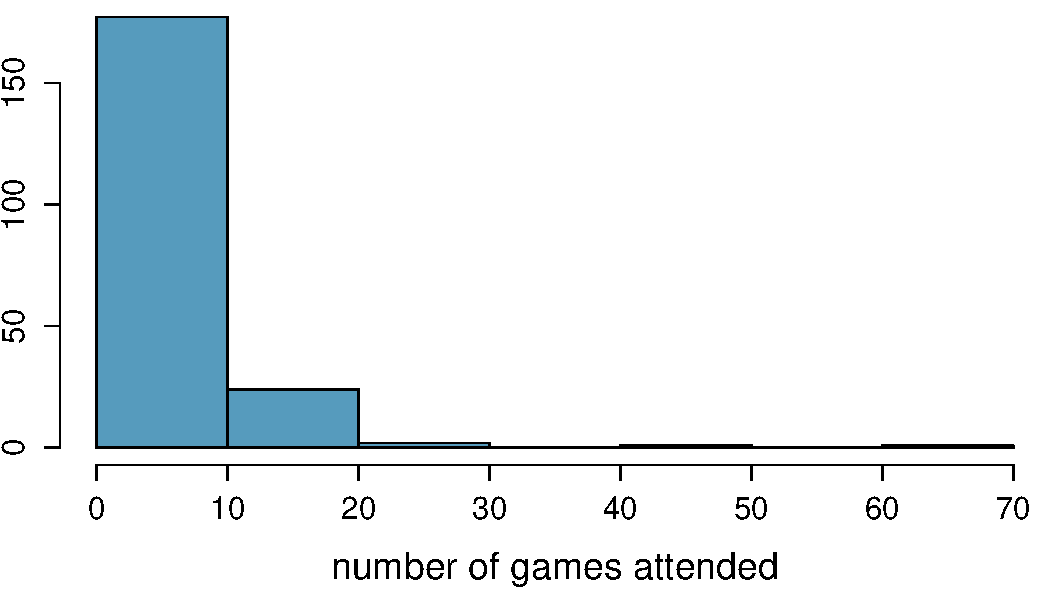
\includegraphics[width=0.8\textwidth]{4-4_clt/figures/duke_games/duke_games_pop}
\end{center}


\end{frame}


%%%%%%%%%%%%%%%%%%%%%%%%%%%%%%%%%%%

\begin{frame}[fragile]
\frametitle{Average number of basketball games attended (cont.)}

Sampling distribution, n = 10:

\twocol{0.6}{0.4}{
\begin{center}
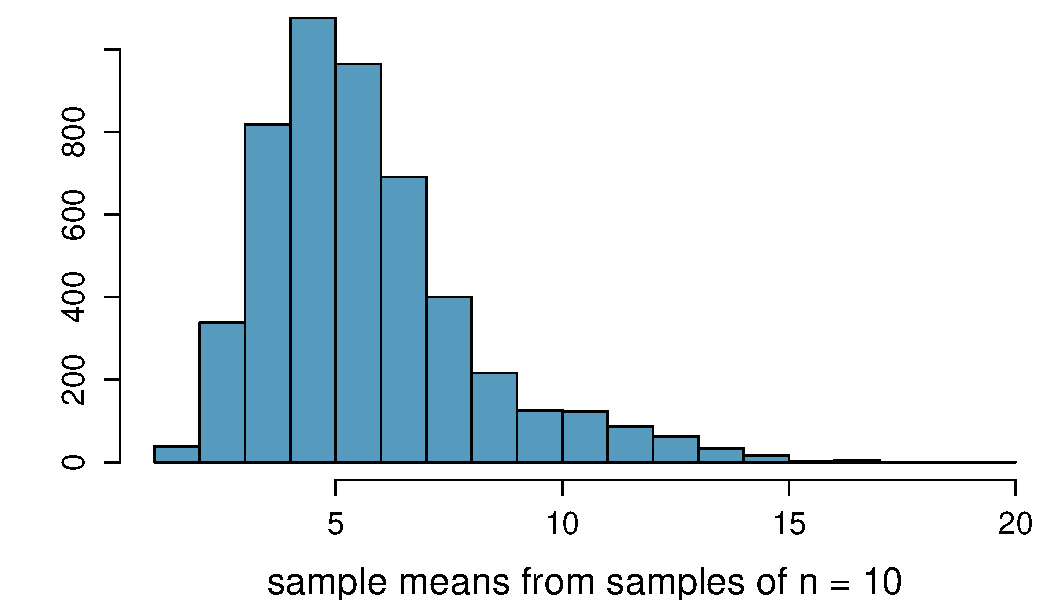
\includegraphics[width=\textwidth]{4-4_clt/figures/duke_games/duke_games_n10}
\end{center}
}
{
\dq{What does each observation in this distribution represent?}
\soln{\only<1>{\textcolor{white}{Sample mean ($\bar{x}$) of samples of size $n = 10$.}}}
\soln{\only<2->{Sample mean ($\bar{x}$) of samples of size $n = 10$.}}
\dq{Is the variability of the sampling distribution smaller or larger than the variability of the population distribution? Why?}
\soln{\only<1-2>{\textcolor{white}{Smaller, sample means will vary less than individual observations.}}}
\soln{\only<3->{Smaller, sample means will vary less than individual observations.}}
}

\end{frame}


%%%%%%%%%%%%%%%%%%%%%%%%%%%%%%%%%%%%

\begin{frame}[fragile]
\frametitle{Average number of basketball games attended (cont.)}

Sampling distribution, n = 30:

\twocol{0.6}{0.4}{
\begin{center}
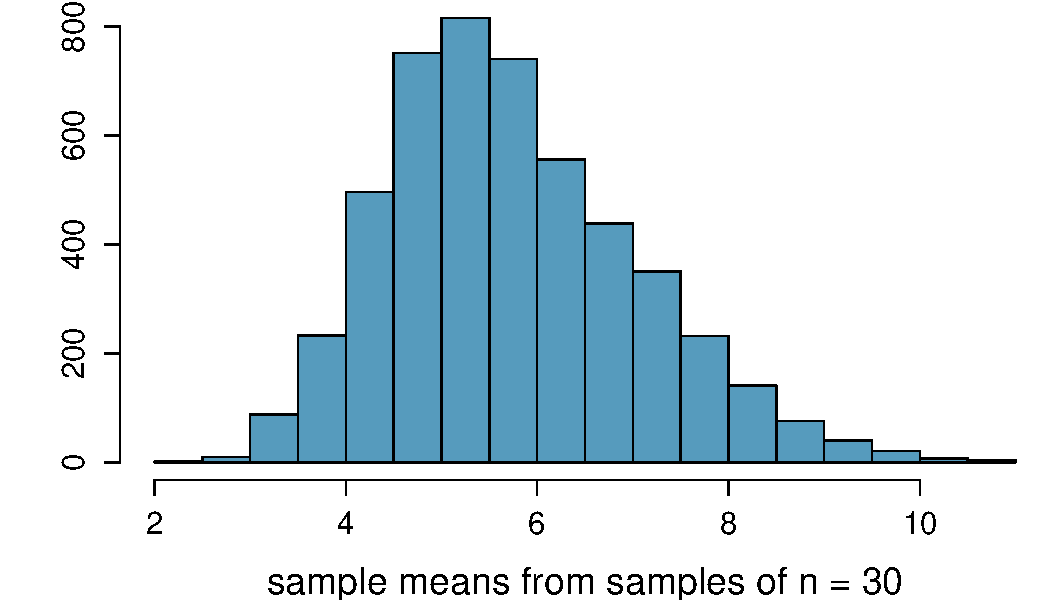
\includegraphics[width=\textwidth]{4-4_clt/figures/duke_games/duke_games_n30}
\end{center}
}
{
\dq{How did the shape, center, and spread of the sampling distribution change going from $n = 10$ to $n = 30$?}
\soln{\only<1>{\textcolor{white}{Shape is more symmetric, center is about the same, spread is smaller.}}}
\soln{\only<2->{Shape is more symmetric, center is about the same, spread is smaller.}}
}

\end{frame}


%%%%%%%%%%%%%%%%%%%%%%%%%%%%%%%%%%%%

\begin{frame}[fragile]
\frametitle{Average number of basketball games attended (cont.)}

Sampling distribution, n = 70:

\begin{center}
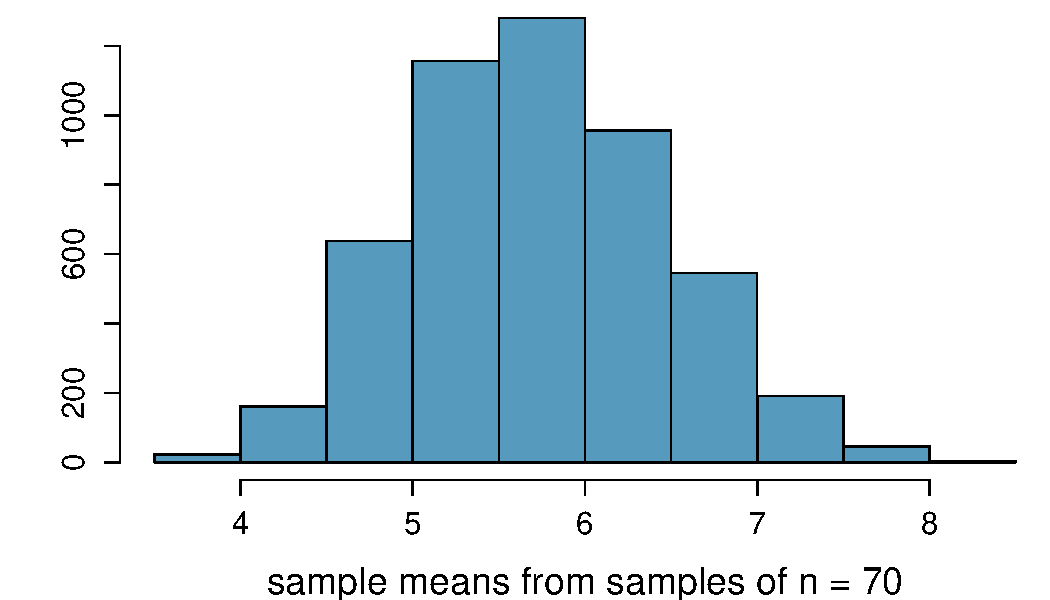
\includegraphics[width=0.6\textwidth]{4-4_clt/figures/duke_games/duke_games_n70}
\end{center}

\end{frame}


%%%%%%%%%%%%%%%%%%%%%%%%%%%%%%%%%%%%

\begin{frame}[fragile]
\frametitle{Average number of basketball games attended (cont.)}

\dq{The mean of the sampling distribution is 5.75, and the standard deviation of the sampling distribution (also called the \hl{standard error}) is 0.75. Which of the following is the most reasonable guess for the 95\% confidence interval for the true average number of basketball games attended by students?}

\begin{enumerate}[(a)]
\item $5.75 \pm 0.75$
\solnMult{$5.75 \pm 2 \times 0.75$} \soln{\only<2>{\red{$\rightarrow (4.25,7.25)$}}}
\item $5.75 \pm 3 \times 0.75$
\item cannot tell from the information given
\end{enumerate}


\end{frame}

%%%%%%%%%%%%%%%%%%%%%%%%%%%%%%%%%%%

\begin{frame}
\frametitle{}

\pq{
{\footnotesize Four plots: Determine which plot (A, B, or C) is which. \\
(1) At top: distribution for a population ($\mu = 10, \sigma = 7$), \\
(2) a single random sample of 100 observations from this population, \\
(3) a distribution of 100 sample means from random samples with size 7, and \\
(4) a distribution of 100 sample means from random samples with size 49.}}

\twocol{0.4}{0.6}{
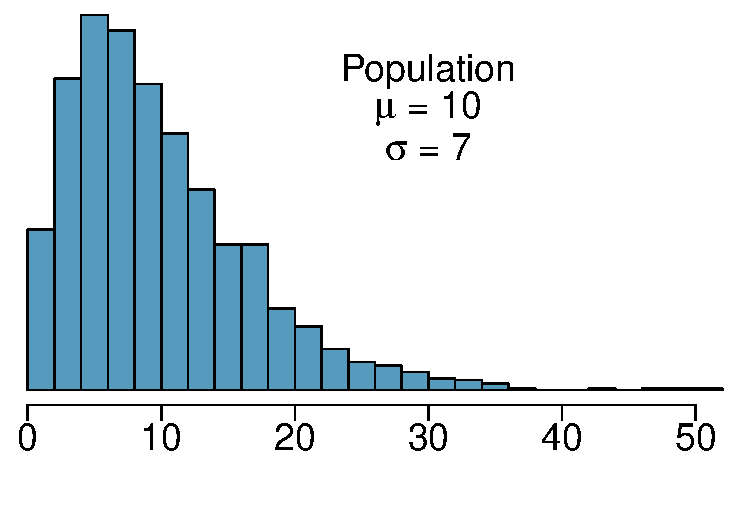
\includegraphics[width=\textwidth]{4-4_clt/figures/cltSimRS/cltSimRS_pop}
}
{
\vspace{-0.5cm}
{\small
\begin{enumerate}[(a)]
\solnMult{A - (3); B - (2); C - (4)}
\item A - (2); B - (3); C - (4)
\item A - (3); B - (4); C - (2)
\item A - (4); B - (2); C - (3)
\end{enumerate}
}
}
\vspace{-0.25cm}
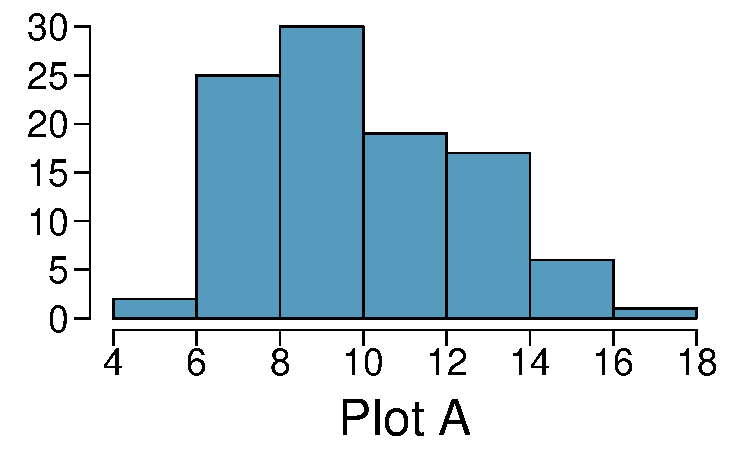
\includegraphics[width=0.32\textwidth]{4-4_clt/figures/cltSimRS/cltSimRS_n7}
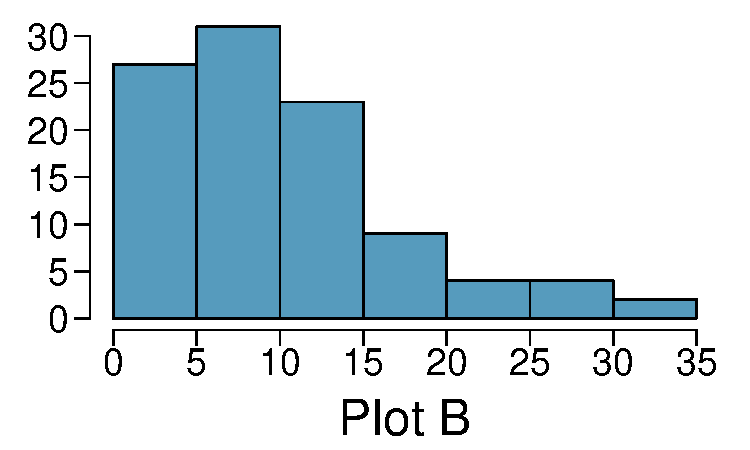
\includegraphics[width=0.32\textwidth]{4-4_clt/figures/cltSimRS/cltSimRS_samp}
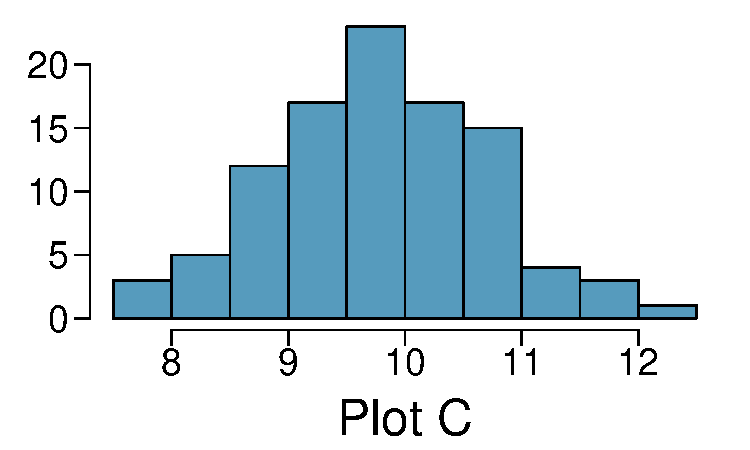
\includegraphics[width=0.32\textwidth]{4-4_clt/figures/cltSimRS/cltSimRS_n49}

\end{frame}

%%%%%%%%%%%%%%%%%%%%%%%%%%%%%%%%%%%%
\section{Inference for other estimators}

%%%%%%%%%%%%%%%%%%%%%%%%%%%%%%%%%%%

\begin{frame}
\frametitle{Inference for other estimators}

\begin{itemize}

\item The sample mean is not the only point estimate for which the sampling distribution is nearly normal. For example, the sampling distribution of sample proportions is also nearly normal when $n$ is sufficiently large.

\item An important assumption about point estimates is that they are \hl{unbiased}, i.e. the sampling distribution of the estimate is centered at the true population parameter it estimates. 
\begin{itemize}
\item That is, an unbiased estimate does not naturally over or underestimate the parameter. Rather, it tends to provide a ``good" estimate. 
\item The sample mean is an example of an unbiased point estimate, as are each of the examples we introduce in this section.
\end{itemize}

\item Some point estimates follow distributions other than the normal distribution, and some scenarios require statistical techniques that we haven't covered yet -- we will discuss these at the end of this section.

\end{itemize}

\end{frame}

%%%%%%%%%%%%%%%%%%%%%%%%%%%%%%%%%%%

\subsection{Confidence intervals for nearly normal point estimates}

%%%%%%%%%%%%%%%%%%%%%%%%%%%%%%%%%%%

\begin{frame}
\frametitle{Confidence intervals for nearly normal point estimates}

A confidence interval based on an unbiased and nearly normal point estimate is

\[ point~estimate � z^\star SE \]

where $z^\star$ is selected to correspond to the confidence level, and SE represents the standard error. 

$\:$ \\

Remember that the value $z^\star SE$ is called the \hl{margin of error}.

\end{frame}

%%%%%%%%%%%%%%%%%%%%%%%%%%%%%%%%%%%

\begin{frame}
\frametitle{}

{\small
\pq{One of the earliest examples of behavioral asymmetry is a preference in humans for turning the head to the right, rather than to the left, during the final weeks of gestation and for the first 6 months after birth. This is thought to influence subsequent development of perceptual and motor preferences. A study of 124 couples found that 64.5\% turned their heads to the right when kissing. The standard error associated with this estimate is roughly 4\%. Which of the below is \emph{false}?}
\begin{enumerate}[(a)]
\solnMult{The 95\% confidence interval for the percentage of kissers who turn their heads to the right is roughly $64.5\% \pm 4\%$.}
\item A higher sample size would yield a lower standard error.
\item The margin of error for a 95\% confidence interval for the percentage of kissers who turn their heads to the right is roughly 8\%.
\item The 99.7\% confidence interval for the percentage of kissers who turn their heads to the right is roughly $64.5\% \pm 12\%$.
\end{enumerate}
}

\vfill

\ct{G\"{u}nt\"{u}rk\"{u}n, O. (2003) Adult persistence of head-turning asymmetry. \textit{Nature}. Vol 421.}

\end{frame}

%%%%%%%%%%%%%%%%%%%%%%%%%%%%%%%%%%%%

\subsection{Hypothesis testing for nearly normal point estimates}

%%%%%%%%%%%%%%%%%%%%%%%%%%%%%%%%%%%

\begin{frame}
\frametitle{Hypothesis testing for nearly normal point estimates}

\dq{The third National Health and Nutrition Examination Survey collected body fat percentage (BF\%) and gender data from 13,601 subjects ages 20 to 80. The average BF\% for the 6,580 men in the sample was 23.9, and this value was 35.0 for the 7,021 women. The standard error for the difference between the average men and women BF\%s was 0.114. Do these data provide convincing evidence that men and women have different average BF\%s. You may assume that the distribution of the point estimate is nearly normal.}

\pause

\begin{enumerate}
\item[1.] Set hypotheses
\item[2.] Calculate point estimate
\item[3.] Check conditions
\item[4.] Draw sampling distribution, shade p-value
\item[5.] Calculate test statistics and p-value, make a decision
\end{enumerate}

\end{frame}

%%%%%%%%%%%%%%%%%%%%%%%%%%%%%%%%%%%

\begin{frame}
\frametitle{}

\begin{enumerate}

\item[1.] The null hypothesis is that men and women have equal average BF\%, and the alternative is that these values are different.
\[ H_0: \mu_{men} = \mu_{women} \qquad H_A: \mu_{men} \ne \mu_{women} \]

\pause

\item [2.]The parameter of interest is the average difference in the population means of BF\%s for men and women, and the point estimate for this parameter is the difference between the two sample means:
\[ \bar{x}_{men} - \bar{x}_{women} = 23.9 - 35.0 = -11.1 \]

\pause

\item[3.] We are assuming that the distribution of the point estimate is nearly normal (we will discuss details for checking this condition in the next chapter, however given the large sample sizes, the normality assumption doesn't seem unwarranted).

\end{enumerate}


\end{frame}

%%%%%%%%%%%%%%%%%%%%%%%%%%%%%%%%%%%

\begin{frame}
\frametitle{}

\begin{enumerate}

\item[4.] The sampling distribution will be centered at the null value ($\mu_{men} - \mu_{women} = 0$), and the p-value is the area beyond the observed difference in sample means in both tails (lower than -11.1 and higher than 11.1).

\begin{center}
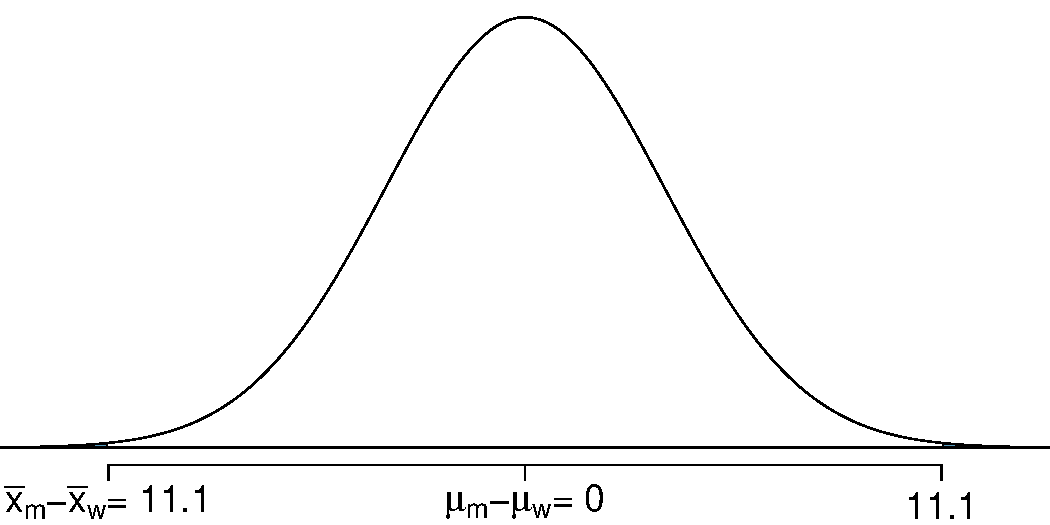
\includegraphics[width=0.75\textwidth]{4-5_inf_other_est/figures/bf/bf}
\end{center}


\end{enumerate}

\end{frame}

%%%%%%%%%%%%%%%%%%%%%%%%%%%%%%%%%%%

\begin{frame}
\frametitle{}

\begin{enumerate}

\item[5.] The test statistic is computed as the difference between the point estimate and the null value (-11.1 - 0 = -11.1), scaled by the standard error.

\[ Z = \frac{11.1 - 0}{0.114} = 97.36 \]

The Z score is huge! And hence the p-value will be tiny, allowing us to reject $H_0$ in favor of $H_A$.

\pause

$\:$ \\

These data provide convincing evidence that the average BF\% of men and women are different.

\end{enumerate}

\end{frame}

%%%%%%%%%%%%%%%%%%%%%%%%%%%%%%%%%%%

\subsection{Non-normal point estimates}

%%%%%%%%%%%%%%%%%%%%%%%%%%%%%%%%%%%

\begin{frame}
\frametitle{Non-normal point estimates}

\begin{itemize}

\item We may apply the ideas of confidence intervals and hypothesis testing to cases where the point estimate or test statistic is not necessarily normal. There are many reasons why such a situation may arise:
\begin{itemize}
\item the sample size is too small for the normal approximation to be valid;
\item the standard error estimate may be poor; or
\item the point estimate tends towards some distribution that is not the normal distribution.
\end{itemize}

\item For each case where the normal approximation is not valid, our first task is always to understand and characterize the sampling distribution of the point estimate or test statistic. Next, we can apply the general frameworks for confidence intervals and hypothesis testing to these alternative distributions.

\end{itemize}

\end{frame}

%%%%%%%%%%%%%%%%%%%%%%%%%%%%%%%%%%%

\subsection{When to retreat}

%%%%%%%%%%%%%%%%%%%%%%%%%%%%%%%%%%%

\begin{frame}
\frametitle{When to retreat}

\begin{itemize}

\item Statistical tools rely on the following two main conditions:
\begin{itemize}
\item \hlGr{Independence} A random sample from less than 10\% of the population ensures independence of observations. In experiments, this is ensured by random assignment. If independence fails, then advanced techniques must be used, and in some such cases, inference may not be possible.
\item \hlGr{Sample size and skew} For example, if the sample size is too small, the skew too strong, or extreme outliers are present, then the normal model for the sample mean will fail.
\end{itemize}

\item Whenever conditions are not satisfied for a statistical technique:
\begin{enumerate}
\item Learn new methods that are appropriate for the data. 
\item Consult a statistician.
\item \sout{Ignore the failure of conditions.} This last option effectively invalidates any analysis and may discredit novel and interesting findings.
\end{enumerate}

\end{itemize}

\end{frame}

%%%%%%%%%%%%%%%%%%%%%%%%%%%%%%%%%%%


%%%%%%%%%%%%%%%%%%%%%%%%%%%%%%%%%%%%
% End document
%%%%%%%%%%%%%%%%%%%%%%%%%%%%%%%%%%%%

\end{document}